\begin{prob}
    Consider this graph:
    \begin{center}
    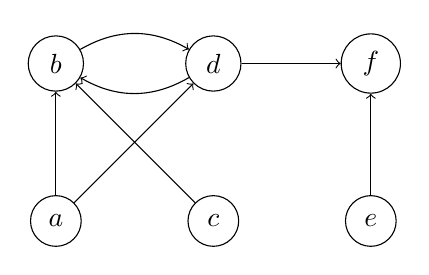
\begin{tikzpicture}
        \tikzset{
            vertex/.style={draw, circle, text width=8, align=center},
            arc/.style={->}
        }

        \draw node[vertex] (a) at (0,0) {$a$};
        \draw node[vertex] (b) at (0,2) {$b$};
        \draw node[vertex] (c) at (2,0) {$c$};
        \draw node[vertex] (d) at (2,2) {$d$};
        \draw node[vertex] (e) at (4,0) {$e$};
        \draw node[vertex] (f) at (4,2) {$f$};

        \foreach \x/\y in {%
            a/b,a/d,d/f,e/f,c/b%
        }{
            \draw (\x) edge[arc] (\y);
        }

        \draw (b) edge[arc, bend left] (d);
        \draw (d) edge[arc, bend left] (b);
    \end{tikzpicture}
    \end{center}

    The questions below will ask you about the properties of this graph. You do
    not need to show work for this problem.

    \begin{subprobset}
        \begin{subprob}
            List four different paths from node $a$ to node $f$. Hint:
            remember that paths do not need to be \emph{simple paths}, that is, a path may visit the same node twice.

            \begin{soln}
                Four possibilities are:
                \begin{align*}
                    &(a,b,d,f),\\ 
                    &(a,d,f),\\
                    &(a,d,b,d,f),\\
                    &(a,d,b,d,b,d,f).
                \end{align*}
                The third path visits $d$ twice -- that's totally fine. The last
                path visits the edges $(b,d)$ and $(d,b)$ twice -- that's also
                fine.

                These aren't the only four paths, since we can come up with infinitely
                many paths from $a$ to $f$ by bouncing back and forth
                between $b$ and $d$. For instance, you could've tried to
                annoy the grader by writing:
                \[
                    (a,b,d,b,d,b,d,b,d,b,d,b,d,b,d,b,d,b,d,f)
                \]
                That's a valid path.
            \end{soln}
        \end{subprob}

        \begin{subprob}
            Recall that a \emph{simple} path is one which has no duplicate nodes;
            that is, it can only visit a node once. List all of the simple
            paths from $a$ to $f$.

            \begin{soln}
                The only simple paths from $a$ to $f$ are:
                \begin{align*}
                    &(a,b,d,f),\\ 
                    &(a,d,f).
                \end{align*}
                The path $(a,d,b,d,f)$ is a valid path, but it is not a \emph{simple}
                path since it visits the node $d$ twice.
            \end{soln}
        \end{subprob}

        \begin{subprob}
            List all of the nodes which are reachable from $a$. Hint: there are four.

            \begin{soln}
                That is, list all of the nodes which are at the end of a path
                which starts at $a$. These are:
                \begin{align*}
                    b,&\quad \text{via, e.g., path $(a,b)$},\\
                    d,&\quad \text{via, e.g., path $(a,d)$},\\
                    f,&\quad \text{via, e.g., path $(a,d,f)$},\\
                    a,&\quad \text{via, e.g., path $(a)$.}
                \end{align*}
                The last one might have been tricky, but remember that every node is reachable from itself.
            \end{soln}
        \end{subprob}

        \begin{subprob}
            What is the total degree of node $b$?

            \begin{soln}
                There are 3 edges coming into $b$, and one edge leaving,
                for a total degree of 4.
            \end{soln}
        \end{subprob}
    \end{subprobset}
\end{prob}
